\chapter{操作系统整体设计} 
% \pagenumbering{arabic} % 阿拉伯数字页码
我将这个简易的操作系统内核命名为RiOS.从结构上看,它实现了系统引导、字符设备驱动、
中断和异常处理、基于连续内存分配的内存管理等,重点实现了文件系统,文件系统部分是
比较完善的.由于水平及时间精力的限制,并没有实现内存分页管理,因而没有缺页调度.
不过它是可扩展的,在此基础上,如果同学们有兴趣,可以尝试分页内存管理并为它加上对多进程
的支持.

\section{操作系统内核引导}
万事开头难,如何正确引导我们的内核,在裸机上打印一行"Hello,world!"是一个简单而又复杂的事.
简单,是因为相对于复杂的内核编写工作它是最简单的;复杂,是因为第一步的跨出需要了解相关背景知识、
面临一些重要的选择,否则将无从下手.

如何加载内核?想象一下上一次装系统的情形,你应该是先将Windows镜像通过软件烧写到U盘中,然后
调整BIOS引导顺序,将U盘启动优先级调到最高,将烧写好的U盘插入电脑,重启,电脑将进入U盘中的Windows
系统.

我们要做的就是得到操作系统内核镜像,用合适版本的gcc编译好自己编写的RiOS内核代码,可以得到内核镜像,
以下工作就和上面一样了.如果你用过"老毛桃"、"大白菜"等软件装过系统,想必对模拟启动功能不陌生.
模拟启动,可以验证是否正确写入,是否能够正常启动,免得我们不断重启白忙一场.编写内核代码不可能一次成功
,我们需要类似模拟启动的功能,QEMU软件就是这样一款广泛使用的虚拟机软件,类似的还有bochs软件,他们性质
类似于Virtualbox或VMware,不过更利于我们调试内核,QEMU广泛应用于国内外的操作系统教学中.

关于引导,我们可以选择是自己写bootloader;也可以像Ubuntu那样使用成熟的GRUB来引导内核.前者我在
之前的实验中查阅相关资料作了初步探索,的确可以引导我们的小内核,但有几个缺点:
\begin{itemize}
    \item 由于x86历史复杂,我们需要背负历史包袱,在代码中要向键盘控制器8042发送命令,打开A20控制器,
这样才能避免地址的回绕,访问到1MB以外的地址.
    \item 因为默认进入的是x86的实模式,(这也是我们在熊老师的汇编语言课上一直使用的模式),我们要进入
保护模式还得费点劲,要清空指令流水线,之后要正确设置GDT表,通过长跳转才能正确进入32位保护模式.
    \item 需要调用BIOS的中断服务程序来将代码从外存拷贝到内存,拷贝过程涉及磁盘的柱面、磁头、扇区,还
需要知道自己U盘的这些参数具体是多少.理论上可以通过查询的方法得到,但之前我为了简单先通过软碟通软件得知这些
参数然后硬编码,这样不利于通用性.
    \item 通过BIOS的中断服务程序调用来拷贝内核,这种方法支持的最大拷贝容量很小,哪怕之后由通过柱面号、
磁头号、扇区号访问的方式改为磁盘LBA访问方式,拷贝容量仍然不是很大.随着代码增长和内核增大,有可能出现
拷贝不完全的现象,内核不能全部加载到内存,将出错.
    \item 以上实现虽然可能只需要一百多行汇编代码,但需要了解相关背景知识,只要有一点写错,就不能成功
引导,代码很难调,关键是我觉得这些与操作系统原理本身关系不是很大,主要是由x86的悠久历史和向后兼容引起的麻烦
,我们没有必要在这上面花费过多时间.    
\end{itemize}
因此在本次课程设计,我选用了GRUB2引导我们的内核,GRUB2也是Ubuntu系统默认的引导方式.这样我们可以专心
内核的编写了.
\subsection{BIOS中断服务程序}
操作系统的引导是从BIOS开始,计算机加电后,BIOS在执行了一系列硬件检测和初始化操作后会将ROM中的64KB代码复制到
内存低端的1M末端的64K处,然后跳转到此地,并让CPU进入实地址模式工作,然后BIOS将会从硬盘或其他块设备将操作系统
引导程序加载到内存0x7c00处,并跳转到这里继续执行引导程序.BIOS会判断我们插入的U盘MBR主引导扇区偏移511处是否为
0x55及偏移512处是否为0xaa,若不满足则认为不可引导,否则将会把它加载到内存0x7c00处.若我们自己编写bootloader,则我们需要确保引导扇区的
代码不超过512字节,我们的整个内核当然会超过512字节,因此需要在这512字节的代码中完成把内核代码全部从外存调入内存的工作.
这里可以使用BIOS中断服务程序,具体可以是BIOS int 13h调用,它是BIOS提供的磁盘基本输入输出中断调用,它可以完成
磁盘读写、校验、格式化等,它历史悠久,采用的是CHS寻址方式,因此最大只能访问8GB左右的硬盘.本课程设计不使用这种方法.
\subsection{GRUB2}
GRUB是GNU GRand Unified Bootloader的缩写,是GNU计划的一个成熟的引导程序包,用它可以实现多操作系统的引导.
这里我们使用GRUB2,只要我们符合多引导头(multiboot header)的规范,它就能将我们带入32位保护模式.
\paragraph{Grub安装到U盘方法}
首先在Ubuntu系统安装grub2,然后插U盘,通过Linux命令安装grub2到U盘
\begin{minted}{shell}
# 首先插入U盘
df -h # U盘是/dev/sdb
sudo mount /dev/sdb /mnt #挂载U盘到/mnt
mkdir /mnt/boot 
sudo grub-install --root-directory=/mnt /dev/sdb
#出现提示错误信息 grub-install: error: will not proceed with blocklists.
#不管他,强制 块列表是不可信赖的,不推荐使用。问题依旧,输入一下指令,强制写入。
sudo grub-install --force --root-directory=/mnt /dev/sdb
\end{minted}
如图~\ref{grub}~所示。

\begin{figure}[!htbp]
	\centering	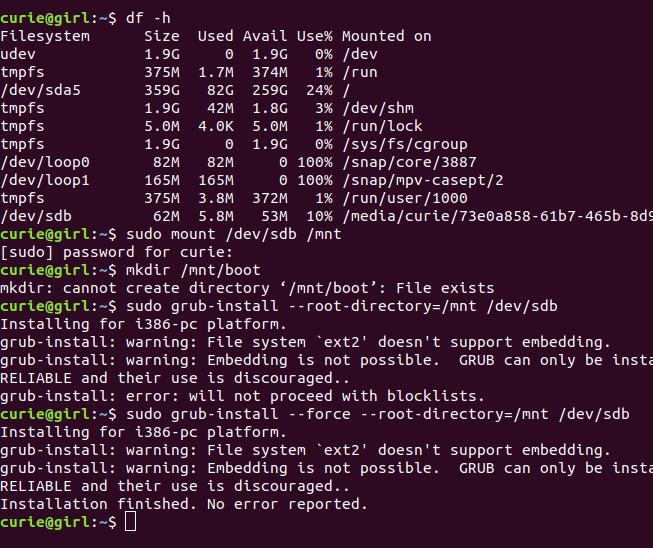
\includegraphics[width=12cm]{pic/assets/grub}
    \caption{grub2安装到U盘过程}	\label{grub}	\end{figure}
Grub的配置文件grub.cfg应当按照相关规范编写,并不困难.
\subsection{Multiboot规范}
Grub引导程序将会检测我们内核是否符合Multiboot头的规范,这里应当查阅相关GNU官方手册,
我们采用较新的Grub2,用到的域有'magic','architecture','header length','checksum'
等几项,对于Grub2,魔法数字(magic)域是32位的0xe85250d6;架构(architecture)域上,我们是
i386保护模式,是0(32位),若是MIPS架构,则这项为4;32位的'checksum'域主要起检查作用,应当保证
'checksum'域和以上的三个域加起来为0,这样Grub才认为Multiboot头正确地写好了.这之后依次还有16位
的'type'域、16位的'flag'域、32位的'size'域,我们令它们分别为0,0,8即可.

\subsection{链接脚本}
我们需要精确控制内核各部分日后加载在内存的位置,因此用来描述输入文件中的各个段(数据段、代码段、堆、栈、bss)
如何映射到输出文件的链接脚本必不可少.链接器是要使用链接脚本的,若不手动提供,它会使用默认的链接脚本.
通过汇编器及gcc编译完我们的诸多代码文件,会得到很多目标文件,通过链接脚本定义的方法,我们将它们有效地组织起来,
最终输出单个的内核镜像.在脚本中,通过OUTPUT\_FORMAT指明输出格式,ENTRY指出入口为boot.asm中
的标号RiOS\_start所在位置.由于CPU低地址有许多预留给系统,故应该把前1MB内存腾出来,内核从1MB后
开始.这部分背景知识可阅读《Linux内核完全注释》.
IBM PC兼容机内存使用如图~\ref{memory}~所示。
\begin{figure}[!htbp]
	\centering	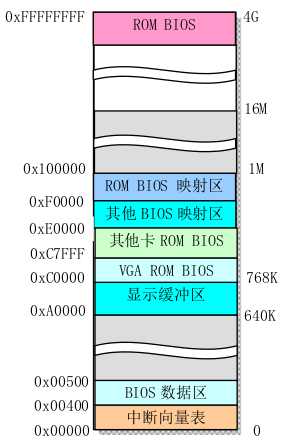
\includegraphics[width=6cm]{pic/assets/memory}
    \caption{内存使用情况}	\label{memory}	\end{figure}

.text区是代码段;.data区是数据段;.bss段则存放那些还没有被初始化的全局变量,BSS是
'Block Started by Symbol Segment'的缩写.

\subsection{Makefile文件}
Makefile是make工具使用时的配置文件,make工具能够自动决定一个含有很多源程序文件的大型程序中哪些文件需要重新编译.
Makefile的使用较为复杂,这里简要介绍一下背景以及本工程的Makefile的编写,关于Makefile的更多写法请阅读GNU make
使用手册.

从Makefile中可以大致看出RiOS的整个框架结构.内核主要由C或C++及汇编构成.在汇编语言课程学习中,我们使用了DOS环境
下MASM汇编器,不过它并不适合我们在Linux环境下交叉编译内核汇编代码.还有很多其他的汇编器,在Linus最初版本的Linux中
,他使用了两种汇编器as86和gas,as86专为Minix和Linux设计,现在应该算过时了,gas是GNU计划的自由软件,作为gcc的一个
后台设计.

本Makefile中使用了grub-mkrescue命令,请确保系统中xorriso已经安装(sudo apt-get install xorriso).

\subsection{汇编器}
我们的RiOS也使用了两种汇编器:NASM和gas.NASM是一个为可移植性和模块化而设计的一个80x86汇编器,
它支持相当多的目标文件格式(包括ELF、a.out、Microsoft 16-bit OBJ等),和Intel语法相似但更简单.(我们在熊老师汇编课上学习的应该算Intel语法)
NASM对宏命令支持相当不错,而且错误检测功能应该优于gas,我们要生成ELF格式的文件,它更加合适.而gas和gcc联系密切,
我们可以较方便地使用内联汇编.因此C编译器采用gcc,汇编器采用NASM及gas,链接器使用ld,另外用make工具完成自动编译.

Makefile中通过.PHONY定义了一些伪目标,比如help、run、clean等,这样make和他们搭配使用,如make help等就能实现相应功能.
内核主要分为内存管理模块、核心模块、块设备模块、字符设备模块、应用层模块等.鉴于之前有编译中间目标文件(.o)过多,和源代码混在一起
,不方便管理的缺点,这次仔细设计内核编译的结构,cd到代码顶层目录第一次敲make时将另外建立build文件夹,将在里面递归建立文件夹,存放中间编译
文件的build文件夹结构组织将和存放代码的src文件夹结构相同,这里使用了Makefile的自动变量功能.这样代码与中间文件分开,结构也比较清晰.

\section{汇编与C的相互调用}
\subsection{从汇编到C语言}
为了减少汇编代码量,提高效率,我们应当尽快过渡到C语言.C语言的函数调用基于栈,只有设置号合适的
函数栈大小和地址,才能有效地实现C语言的函数调用.在之前的计算机图形学课程中的种子填充算法中,我们体验过
栈溢出导致的程序崩溃,所以考虑到有些函数将使用较多的栈空间,我们不应吝惜开始预留的栈空间.内核编写中,
有过这样的体验:当函数调用空间消耗较大时,莫名其妙内核崩溃了,但从代码上找不出任何逻辑错误.栈预留16KB可能
差不多了,但为了避免"stackoverflow"的悲剧,我预留了16MB.关中断,然后将esp指向要设置的栈顶位置,再通过
call调用C语言里编写的RiOS\_main函数去.这里的call应是一去不复返了.这样就完成了汇编到C语言的切换.
通过汇编mov指令或者是通过C语言的指针写显存,我们都可以在屏幕打印字符,将内核复制到装有grub的U盘指定位置,
插入U盘,调整启动顺序,计算机重启可以进入U盘中的内核,实现裸机的Hello,World.
Hello,World 如图~\ref{hello}~所示。
\begin{figure}[!htbp]
	\centering	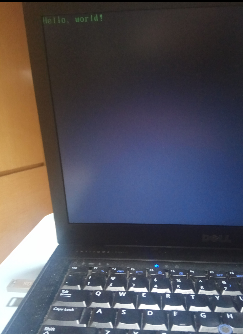
\includegraphics[width=6cm]{pic/assets/hello}
    \caption{裸机上的Hello,World!}	\label{hello}	\end{figure}
\subsection{从C到C++}
我们已经从汇编进入C语言,但是我们如何使用C++语言呢?在之前的实验中,我的探索失败了,当时我发现汇编调用不了C++
的代码,把C++代码反汇编过来会发现,与C语言不一样的是:若C语言中写一个名为foo的函数,反汇编过来是foo的标号,
而在C++中这样做则会在foo这个标号加上前缀后缀.因此若在汇编代码中调用foo函数,用foo标号按图索骥在C语言行得通,
而C++由于标号变了,就会出现'undefined'的错误.

要解决这个问题不难,但我知识浅薄,之后才发现,我应当使用在函数声明中使用extern "C".这样C++才可以调用其他C
语言代码.加上extern "C"后,会指示编译器将这部分代码按C语言的进行编译,而不是C++的.请注意是函数的声明,
不是函数的定义,因此 extern "C"主要放在头文件内.这样一来,就可以方便地使用类了.然而对于开发简易内核的我们,
使用C++可能并不是一个很好的选择.不要高兴太早,真正完全的C++的支持需要操作系统帮忙,比如异常是用不了的,它要求
运行时的支持以及内存管理的支持.类的构造和析构应该也需要内存管理的支持,然而刚刚引导时,我们尚未写相关代码,这是
个先有鸡还是先有蛋的问题.C语言更适合底层,Linux内核编写也选择的是C语言而不是C++,在此我只是探索,实际也还是
C语言风格,并未用到很多C++特性.
\paragraph{*.CC文件} 你可能注意到代码中大部分是.cc后缀的代码文件,这和我们熟知的.cpp文件其实是一样的.cc文件是Linux/UNIX下
为C++源文件默认的扩展名,不过请还是不要将它改为cpp文件,否则gcc可能不能正确识别.
\paragraph{汇编语言} 虽然在汇编语言课程中已经学过汇编语言,然而光了解8086汇编是远远不够的,386以后体系结构有所
变化,要编写面向x86(i386以后)的内核,应当了解这部分背景知识,包括之后在8086基础上新增的段寄存器等.

\section{段描述符}
bootloader接手BIOS后,开始PC系统处于16位的实模式,若自己写bootloader,还有一个切换的过程,而现在GRUB将直接把内核带
入32位保护模式.只要在32位保护模式下,才能突破实模式可使用物理内存空间不超过1MB的限制,最多可管理4GB内存;才能使用分段存储
管理机制.分段机制涉及这几方面内容:逻辑地址、段描述符(描述段的属性)、段描述符表、段选择子.

段选择子涉及段寄存器,用于定位段描述符表中表项的索引.段描述符表是段描述符的一个数组,段描述符表的长度可变,最多可包含8192个8字节描述符.有两种描述符表
:全局描述符表GDT和局部描述符表IDT.
\subsection{全局描述符表GDT (Global Descriptor Table)}

GDT本身只是线性地址空间中的一个数据结构,GDT的基线性地址和长度值必须加载进GDTR寄存器中.
GDT的基地址应当是内存8字节对齐的.《从实模式到保护模式》一书中给出了存储器的
段描述符格式:见图~\ref{gdt}~.

\begin{figure}[!htbp]
	\centering	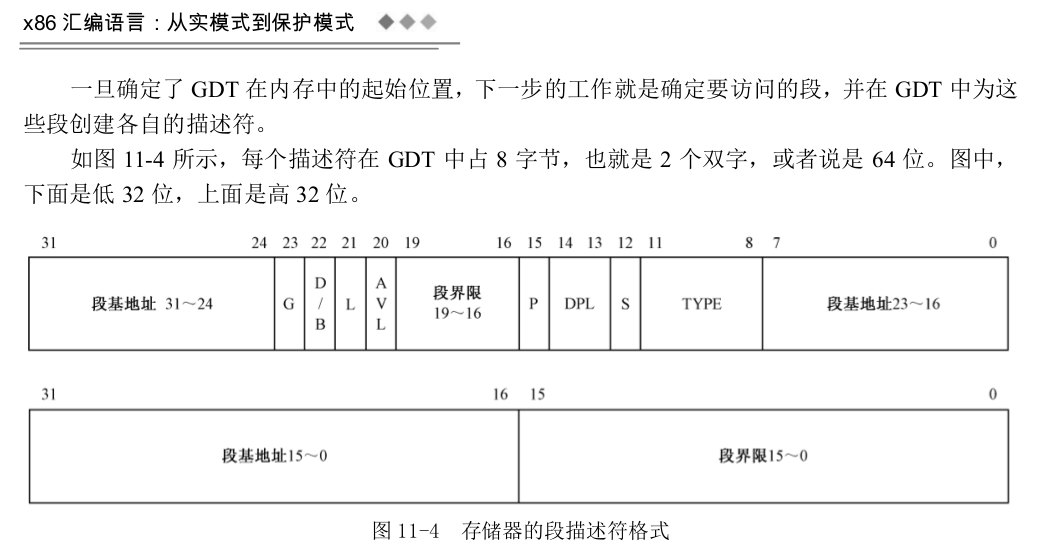
\includegraphics[width=14cm]{pic/assets/gdt}
    \caption{段描述符格式}	\label{gdt}	\end{figure}

段描述符这个格式比较复杂,一部分原因是x86历史较长,为了后向兼容,有时一个简单的
数据项往往要拆成几处,这样看起来就比较乱了,不过写代码时要严格按照硬件上的结构来,
不能出现哪怕一位的差错.



再来一个类似的段描述符结构的图:如图~\ref{segment_descriptor}~所示

\begin{figure}[!htbp]
	\centering	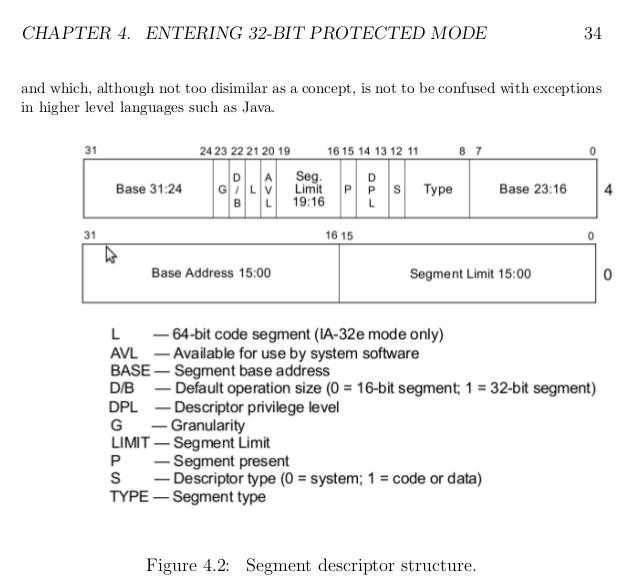
\includegraphics[width=14cm]{pic/assets/segment_descriptor}
    \caption{段描述符的结构}	\label{segment_descriptor}	\end{figure}


GDT表中的一项是64位(8B);而GDTR寄存器用来存放全局描述符表32位线性地址和
16位表长度值,故GDTR长度是48位.关于GDT及GDTR的介绍可见维基百科Global\underline{ }Descriptor
\_Table词条,亦可见《LInux内核完全剖析》76页介绍,图~\ref{wiki_gdt}~为48位的GDTR的结构.
\begin{figure}[!htbp]
	\centering	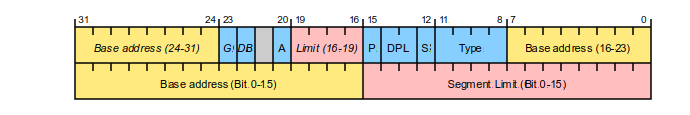
\includegraphics[width=14cm]{pic/assets/wiki_gdt}
    \caption{GDTR寄存器的结构}	\label{wiki_gdt}	\end{figure}
   
对应以上结构,RiOS中GDT表项的结构如下:
\begin{minted}{c}
struct GDT_entry 
{
u16 limit1;      /*0-15*/		
u16 base1;       /*16-31*/
u8 base2;        /*32-39*/
u8 access;       /*40-47*/
u8 granularity;  /*48-55*/
u8 base3;        /*56-63*/
} __attribute__((packed));  
\end{minted}    
GDT表项是64位,但是GDTR寄存器是48位,我们需要lgdt(Load GDT Register)
指令加载全局描述符表寄存器GDTR,把GDT表的基地址和长度从内存加载到GDTR中.
RiOS中GDT\_pointer结构由基地址和长度组成.将在RiOS/src/kernel/gas/gdt.S
中的update\_gdt函数用一条汇编指令lgdt (gdt\_pointer)完成加载到GDTR的工作.
\begin{minted}{c}
struct GDT_pointer
{
u16 limit;
u32 base;
} __attribute__((packed));
\end{minted}  

举一个段间长跳转的例子,例如用AT\&T语法写(gas)是
\mintinline{gas}!ljmp $section, $offset!

,而intel语法为
\mintinline{asm}!jmp section:offset!
.具体如
\mintinline{nasm}!ljmp $0x8, $protcseg!
,ljmp的格式是: ljmp 段选择子,段内偏移.上句指令的意思是:用0x8作为段选择符,
到gdt中去取出gdt[0x8]的值,再加上偏移量protcseg. 跳转到gdt[0x8] + \$protcseg
的地址处执行。 
\subsection{局部描述符表LDT (Local Descriptor Table)}
发生任务切换时,LDT会更换成新任务的LDT,但GDT不会改变.由于时间精力有限,本项目目前并未涉及,但
日后若要加入对多任务和虚拟内存的支持,应当研究好这一块.
\section{中断描述符表IDT (Interrupt Descriptor Table)}
在保护模式下,中断门描述符表(IDT)中断每个表项由8个字节组成,其中每个表项叫做一个门描述符
(Gate Descriptor).在IDT中,可以包含如下几种类型的系统段描述符:
\begin{itemize}
    \item 中断门描述符(Interrupt-gate descriptor)
    \item 陷阱门描述符(Trap-gate descriptor)
    \item 任务门描述符(Task-gate descriptor)和调用门描述符(Call-gate descriptor)
\end{itemize}
其中中断门描述符和陷阱门描述符的类型码分别为110和111.

\subsection{门描述符}
以下为RiOS中门描述符的数据结构,以上几种门描述符都可以是这种类型.这里使用\mintinline{gas}!
#pragma pack(1)!设置结构体的边界对齐为1个字节,也就是所有数据在内存中是连续存储的,因为这和硬件直接相关,需要精确控制到"位".
\begin{minted}{c}
#pragma pack(1)
struct GATE_DESCRPTOR{
u16 offset_lowerbits        :16;// offset bits 0..15
u16 selector                :16;// a code segment selector in GDT or LDT
u8  zero                    :8 ;// unused,set to 0
// type and attributes, total u8 type_attr;
u8  seg_type                :4 ;
u8  storage                 :1; // set to 0 for interrupt and trap gates 
u8  descr_privilege_level   :2;
u8  present                 :1;
u16 offset_higherbits       :16;// offset bits 16..31	
};
#pragma pack()
\end{minted}

中断描述符表的前32项应当留给处理器内部的异常处理.80386把中断号0至31分配
给陷阱、故障和不可屏蔽中断,把32至47之间的中断号分配给可屏蔽中断。
可屏蔽中断的中断号是通过对中断控制器的编程来设置的。

\begin{tabular}{|c|c|c|}% 通过添加 | 来表示是否需要绘制竖线
    \toprule
    Exception \# & Description & Error Code?\tabularnewline
    \midrule
    0 & Division By Zero Exception & No\tabularnewline
    1 & Debug Exception & No\tabularnewline
    2 & Non Maskable Interrupt Exception & No\tabularnewline
    3 & Breakpoint Exception & No\tabularnewline
    4 & Into Detected Overflow Exception & No\tabularnewline
    5 & Out of Bounds Exception & No\tabularnewline
    6 & Invalid Opcode Exception & No\tabularnewline
    7 & No Coprocessor Exception & No\tabularnewline
    8 & Double Fault Exception & Yes\tabularnewline
    9 & Coprocessor Segment Overrun Exception & No\tabularnewline
    10 & Bad TSS Exception & Yes\tabularnewline
    11 & Segment Not Present Exception & Yes\tabularnewline
    12 & Stack Fault Exception & Yes\tabularnewline
    13 & General Protection Fault Exception & Yes\tabularnewline
    14 & Page Fault Exception & Yes\tabularnewline
    15 & Unknown Interrupt Exception & No\tabularnewline
    16 & Coprocessor Fault Exception & No\tabularnewline
    17 & Alignment Check Exception (486+) & No\tabularnewline
    18 & Machine Check Exception (Pentium/586+) & No\tabularnewline
    19 to 31 & Reserved Exceptions &\tabularnewline
    \bottomrule
\end{tabular}

以上为0到31号分配给陷阱、故障和不可屏蔽中断的具体情况,这部分编写和中断类似,
举一个除0异常的例子,代码中出现除以0的情况,将会陷入系统异常的处理例程,系统发生panic,
打印出错信息,内核停机(halt).

如图~\ref{divisionbyzero}~.

\begin{figure}[!htbp]
	\centering	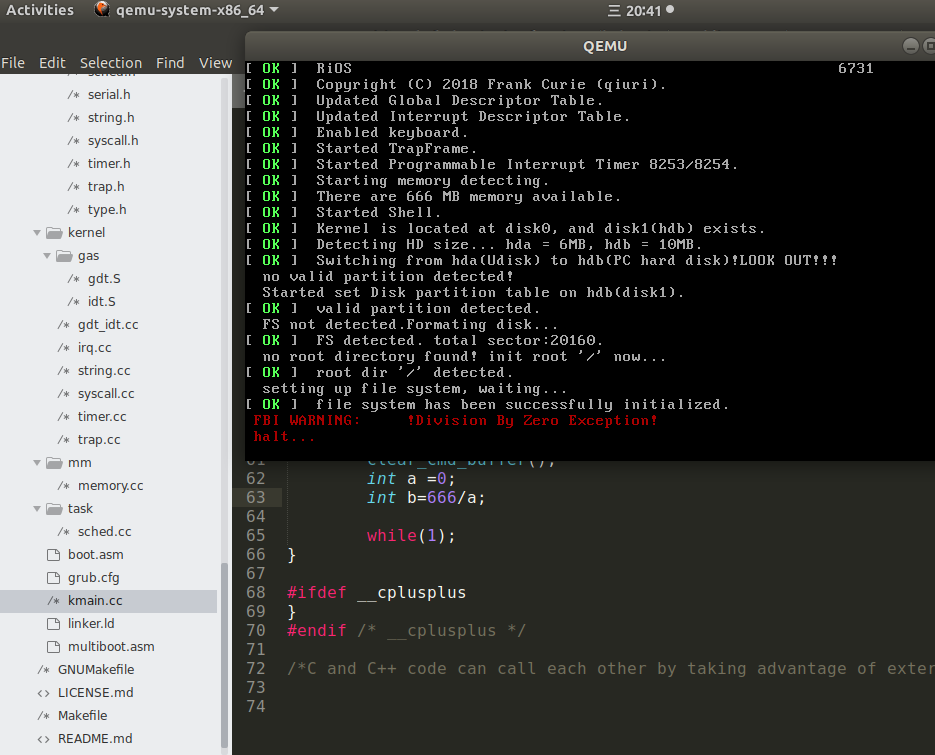
\includegraphics[width=14cm]{pic/assets/divisionbyzero}
    \caption{除0异常}	\label{divisionbyzero}	\end{figure}

IDT表中的项类似于GDT表中的项,它们都是64位长,都有基地址,都有访问标志位;然而IDT没有类似
GDT中的段限长(limit).

如图~\ref{interrupt_trap_gate}~.

\begin{figure}[!htbp]
	\centering	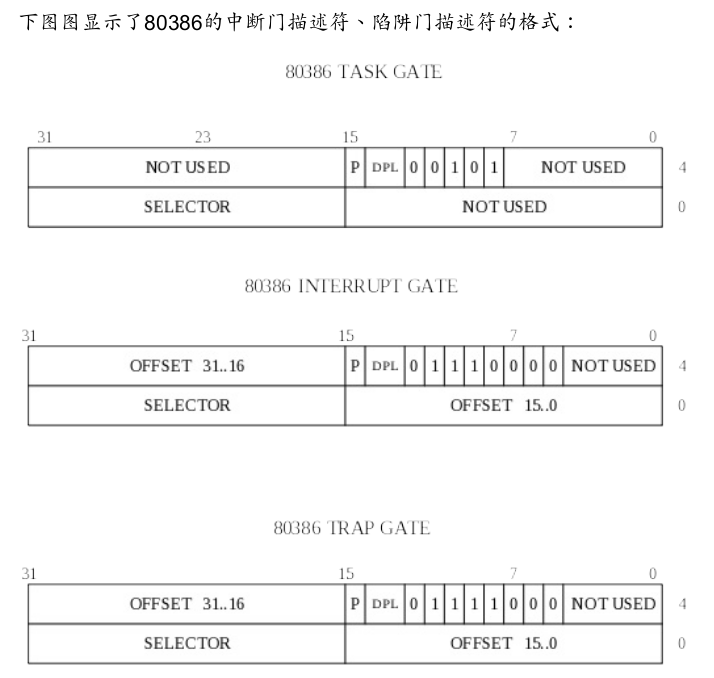
\includegraphics[width=14cm]{pic/assets/interrupt_trap_gate}
    \caption{门描述符1}	\label{interrupt_trap_gate}	\end{figure}

其他资料上类似的还有图~\ref{IDT_Gate_descriptors}~.
\begin{figure}[!htbp]
        \centering	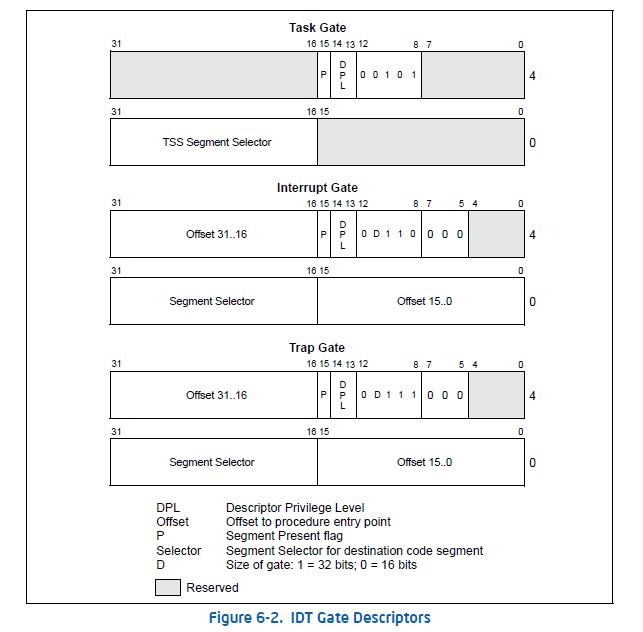
\includegraphics[width=14cm]{pic/assets/IDT_Gate_descriptors}
        \caption{门描述符2}	\label{IDT_Gate_descriptors}	\end{figure}

我们的IDT表设置了256项,当触发中断的条件满足,将会利用中断向量号查IDT表,然后转入相应
的中断服务程序,处理完再返回.如果考虑不严密,将会出现这样的情况:尚未写某个中断的处理程序,
然而相应中断或异常发生,查IDT表不知道转入到什么地方执行了,系统会因此崩溃,具体体现就是
只要这个中断触发,就会无限循环地重启.为避免这种情况发生,我们可以先把所有256项都填满,
先占个坑位;对于尚未编写的中断,统一转到一个什么也不干的中断服务程序(汇编语言编写的idt.S中的
asm\_all\_trap函数).每当我们实现一个新的服务函数,才做出相应修改,转到新写的函数中.
这部分需要把汇编语言编写的idt.S、gdt.S及用宏定义包装汇编以便于C语言调用的头文件x86.h结合起来看.
这里使用了一些汇编语言和C语言或C++相互调用的小技巧,另外需要理解栈帧的相关概念.



\paragraph{键盘中断服务程序}

\section{栈帧}
数据结构课程中的栈在硬件也有体现,x86CPU架构有专门的'push'、'pop'指令来完成入栈出栈的
操作.在x86中栈是向下增长的满栈(full descending stack),C语言的函数调用离不开
栈,GCC编译器规定的函数栈帧(stack frame)是一块存放某函数的局部变量、参数、返回地址
和其他临时变量的内存空间,图~\ref{stackframe}~为栈帧的大致结构.
\begin{figure}[!htbp]
    \centering	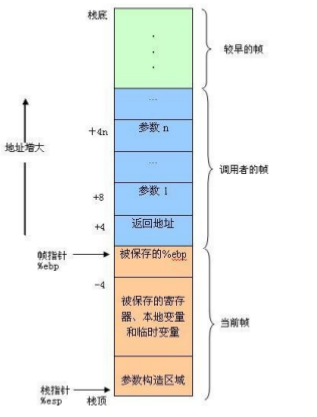
\includegraphics[width=6cm]{pic/assets/stackframe}
    \caption{栈帧结构}	\label{stackframe}	\end{figure}

\subsection{内核栈上的陷阱帧(TrapFrame)}
RiOS中的陷阱帧结构如下:
\begin{minted}{c}
struct TrapFrame{
/*registers that pushed by "pushal",xxxesp is useless */	
  u32 edi,esi,ebp,xxxesp,ebx,edx,ecx,eax;
/*below are defined by x86 hardware:eip cs .. eflags*/
  u32 err;/*irq*/
  u32 eip; 
  u16 cs; u16 padding;
  u32 eflags;
};
\end{minted}
为什么会这样?这里要先分析一下中断处理过程:

中断发生以后,CPU在通过查询IDT表跳转到中断处理例程之前,将在内核栈中依次压入错误码
(可选)、eip、CS和EFLAGS,这对应RiOS中TrapFrame结构的err、eip、cs和padding(因为字节对齐)、
eflags,其中err对应的错误码是我们手动压入的,通过不一样的错误码,可以判别到底发生何种错误.
而后面3个为x86硬件决定,顺序也是定死了的.中断后内核栈发生了变化,可以看到RiOS里一些函数以
TrapFrame结构体为传入参数,例如
\mintinline{asm}!void irq_handle(TrapFrame *trapframe);!
C语言函数传参就是通过栈实现的.这样他们可以从内核栈中把压入栈的TrapFrame"掏"出来使用.
中断发生时,将通过查IDT表跳转到各个中断对应的中断处理程序,就是在汇编写成的RiOS/src/kernel
/gas/idt.S定义的一堆名字中带handler的程序,这些handler各自压入独特错误码,然后统一转入asm\_
all\_trap函数.这仿佛一个陷阱,把所有handler都栽进去了,asm\_all\_trap到底做了什么?
\begin{minted}{gas}
asm_all_trap:
    pushal 
    push %esp
    call irq_handle
    pop %esp
    popal
    add $4,%esp
    iret
\end{minted}
可见它先pushal,先把很多寄存器的值压入栈,注意这对应TrapFrame结构的edi、esi、ebp、xxxesp、ebx、edx、ecx、eax
.另外此处的xxxesp并没有什么用.中断过程我们要密切关注栈里到底压入了什么.asm\_all\_trap这样写的目的就在于
,通过给栈中压寄存器们的值,使内核栈看起来就好像压入了一个陷阱帧结构,这样那些函数才能够从栈中
"掏出"陷阱帧.call irq\_handle函数以后,转入RiOS/src/kernel/trap.cc中的C语言函数,此函数
判断栈中的(或者说传入的参数)陷阱帧的标志码(err)是多少,然后转入相应的中断处理函数.

由于时间精力的限制,我没有写进程切换,不过基础设施已经大致搭好.日后同学们若要实现多进程,应当把中断处理过程分析清楚.
在trap.cc中的irq\_handle函数中timer\_8253\_handler\_main函数是时钟中断的处理函数,它包着do\_timer函数,进程调度
就应该改写do\_timer函数,在里面进行进程切换.

call irq\_handle以后转入irq\_handle根据err值执行不同中断服务程序,运行完还回到asm\_all\_trap,做中断最后
的恢复现场工作,既然之前
\mintinline{gas}!pushal push %esp!
,那么现在就要
\mintinline{gas}!pop %esp popal!
.为何要add \$4呢?别忘了,之前idt.S里那些一群handler们可是先压入了独特的标志码(err)的,那么现在要
恢复内核栈就要加回来.如果你之前还想再多压一些信息进栈,这里就要多加.总之,这是一个对称的过程,目的是恢复内核栈.

\section{字符设备驱动}
\subsection{屏幕}
\paragraph{光标的设置} 光标跟随输入的字符而移动,这件事不是天经地义的,它的实现也需要我们写相关代码.
VGA显卡内部有一系列寄存器可以用来控制显卡的状态。在标准的PC机上,
0x3d4和0x3d5两个端口可以用来读写显卡的内部寄存器。方法是先向0x3d4端口写入要访问的寄存器编号,
再通过0x3d5端口来读写寄存器数据。存放光标位置的寄存器编号为14和15。两个寄存器合起来组成一个16位整数,
这个整数就是光标的位置。比如0表示光标在第0行第0列,81表示第1行第1列(屏幕总共80列)。 
以下代码截取的是RiOS/src/console/console.cc中set\_cursor函数的代码,用于设置光标.

\begin{minted}{c}
Vx = xyindex%80;
Vy = xyindex/80;
u16 tmp = (Vy*80)+Vx;
outb(0x3d4,0x0f);
outb(0x3d5,(u8)(tmp & 0xff));/*cursor low port:reg15*/
outb(0x3d4,0x0e);
outb(0x3d5,(u8)( (tmp >> 8) & 0xff));/*cursor high port:reg14*/
\end{minted}    
\subsection{键盘}
\section{定时器(8253芯片或其兼容芯片)的设置}

微机原理课程学完之后不知道有什么用处,当我写本项目时才觉得还是有用的.
8253芯片和8259芯片的设置在本实验中都要用到,这里用宏定义或内联汇编把
in、out指令包装起来在C语言中用,实际上还是微机原理的那一套,初始化字
的写入等可以查阅相关资料,这里不详细展开了.

8253的初始化设置如下.
\begin{minted}{c}
void init_8253()
{
	outb(PIT_COMMAND_REG,0x34);
/*bin(0x34)='0b110100'= 00   11    010   0
 *Channel 0 ,Access mode: lobyte/hibyte , Mode 2 (rate generator),16-bit binary 
 */	
	outb(PIT_CHANNEL0_DATA_PORT,0x9c);/*low byte*/
	outb(PIT_CHANNEL0_DATA_PORT,0x2e);/*high byte*/
/* 1193180/100 = 11930 ,100HZ => a irq every 10ms
 * 11930 = 0b 0010 1110 1001 1010,first write lower bits,then the higher
 * see my guide.md and https://wiki.osdev.org/Programmable_Interval_Timer
 */	
	enable_8253();
	msg_8253_ok();
}
\end{minted}    
\section{块设备驱动}
操作系统需要和周边的输入输出设备通信,"存储程序,程序控制",操作系统应当具有管理和存储
长期保存数据的软件功能,这就是文件系统.文件系统不是空中楼阁,必须先对硬件进行封装,
这就是块设备驱动程序的意义.

使用fopen、fprintf不是很简单吗?然而这是所在的操作系统给我们封装好的库函数,我们在
实现一个简易操作系统内核,所有这些库函数都是不能用的,我们需要从底层往上逐步实现他们.
离开这些库函数,我们还能怎样操纵硬盘,读取写入数据?

I/O控制方式有:轮询方式、中断方式、DMA方式、通道方式.嵌入式系统这类课程常常会谈到"串口",原因就在于"串口"相对比较简单.
x86架构下,我们还有in、out指令来操纵外设,操纵外设需要了解外设与CPU通信的协议,高级点的我们做不了,就采用简单的中断方式,
使用in out指令来完成对硬盘的读写.
图~\ref{ports}~为常见的端口地址.来自百度百科词条"寻址空间"下'端口地址分配'
\begin{figure}[!htbp]
    \centering	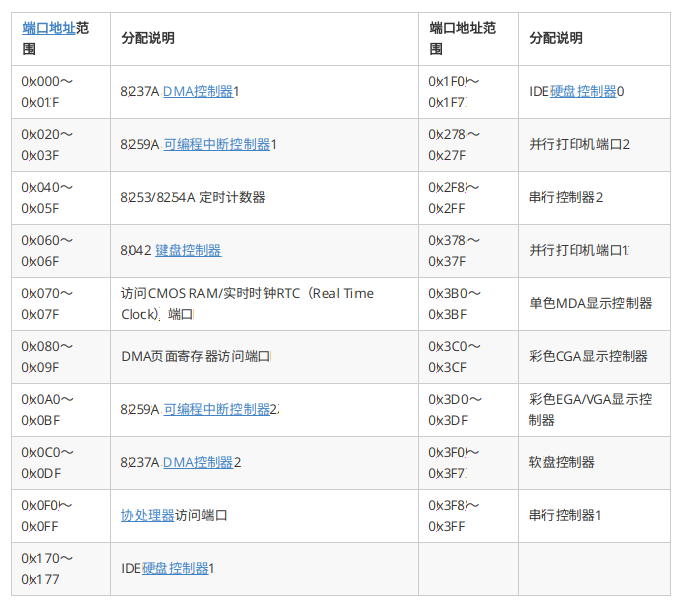
\includegraphics[width=12cm]{pic/assets/ports}
    \caption{端口地址分配}	\label{ports}	\end{figure}

其中端口0x1F0至0x1F7用于IDE硬盘控制器0,写IDE硬盘驱动主要用到它.

\subsection{IDE(ATA)硬盘}
这是一种规范,大多数情况下,IDE和ATA是同义词,IDE用得多一点,但实际上叫ATA可能更合理.
注意,这里我们讨论的是硬盘方面的IDE,并不是讨论集成开发环境的那个IDE.
以下是来自osdev网站的相关介绍(https://wiki.osdev.org/Category:ATA):

The name IDE is often used interchangeably with ATA, but "IDE" actually refers to only the 
electrical specifications of the signals on the 40 / 80 pin disk cable. ATA is the proper 
name for the entire specification.


\section{文件系统设计与实现}
下一章详细说明.


% \section{引用示例}

% \section{引用示例}
% \subsection{垃圾}
% 垃圾

% \section{引用示例}

% \clearpage